\section{Auswertung}
\label{sec:Auswertung}


Die Graphen werden sowohl mit Matplotlib \cite{matplotlib} als auch NumPy \cite{numpy} erstellt. Die Fehlerrechnung wird mithilfe von Uncertainties \cite{uncertainties} durchgeführt.

\subsection{Elektronen im E-Feld}
\subsubsection{Empfindlichkeiten}
In Tabelle \ref{tab:Elek} sind die Messwerte für die Ablenkspannungen $U_.d$ für eine Ablenkung $D$ benötigt werden bei den Beschleunigungsspannungen
\begin{align*}
U_.B&=\SI{310}{\volt},\\
&=\SI{280}{\volt},\\
&=\SI{260}{\volt},\\
&=\SI{240}{\volt},\\
&=\SI{220}{\volt}
\end{align*}
zu finden. Die mittels der linearen Regression $D(U_.d)=\alpha U_.d + \beta$ bestimmten Graphen sind in Abbildung \ref{fig:Elek} zu sehen.
Es ergeben sich die Parameter
\begin{align*}
\alpha_.{310}&=\SI{1,050(6)e-3}{\metre\per\volt},\\
\alpha_.{280}&=\SI{1,146(5)e-3}{\metre\per\volt},\\
\alpha_.{260}&=\SI{1,227(9)e-3}{\metre\per\volt},\\
\alpha_.{240}&=\SI{1,338(12)e-3}{\metre\per\volt},\\
\alpha_.{220}&=\SI{1,460(12)e-3}{\metre\per\volt},\\
\beta_.{310}&=\SI{-11,19(11)e-3}{\metre},\\
\beta_.{280}&=\SI{-10,45(9)e-3}{\metre},\\
\beta_.{260}&=\SI{-9,93(14)e-3}{\metre},\\
\beta_.{240}&=\SI{-10,11(16)e-3}{\metre},\\
\beta_.{220}&=\SI{-9,83(15)e-3}{\metre}
\end{align*}
In Abbildung \ref{fig:Elek2} sind die Empfindlichkeiten $\alpha$ gegen $\frac{1}{U_.B}$ aufgetragen.
Eine lineare Ausgleichsrechnung der Form
$\alpha\left(\frac{1}{U_.B}\right)=a\cdot\frac{1}{U_.B}+b$
ergibt die Parameter
\begin{align*}
a&=\SI{0,313(8)}{\metre},\\
b&=\SI{3,3(31)e-5}{\metre\per\volt}
\end{align*}
Der Theoriewert für die Steigung ergibt sich nach Formel \eqref{eq:} zu
\[
a_.{theo}=\SI{0,204}{\metre}
\]
\begin{table}
\centering
\caption{Messwerte der Ablenkspannungen bei verschiedenen Beschleunigungsspannungen $U_.B$}
\label{tab:tabElek}
	\sisetup{table-format=1.2}
	\begin{tabular}{S[table-format=2.2]S[table-format=2.1]S[table-format=2.1]S[table-format=2.1]S[table-format=2.1]S[table-format=2.1]}
		\toprule
		{$D/\si{\metre}$} & {$U_.{d,310}/\si{\volt}$} & {$U_.{d,280}/\si{\volt}$} & {$U_.{d,260}/\si{\volt}$} & {$U_.{d,240}/\si{\volt}$} & {$U_.{d,220}/\si{\volt}$} \\
		\midrule
		25.00 & 34.0 & 30.7 & 28.0 & 25.7 & 23.5 \\
		18.75 & 28.5 & 25.4 & 23.3 & 21.6 & 19.4 \\
		12.50 & 22.8 & 20.2 & 18.4 & 17.1 & 15.5 \\
		6.25 & 16.8 & 14.7 & 13.5 & 12.3 & 11.3 \\
		-0.00 & 10.9 & 9.2 & 8.4 & 8.0 & 6.9 \\
		-6.25 & 4.8 & 3.8 & 3.3 & 3.1 & 2.6 \\
		-12.50 & -1.2 & -1.6 & -2.2 & -1.8 & -1.6 \\
		-18.75 & -7.3 & -7.5 & -7.4 & -6.6 & -6.3 \\
		-25.00 & -13.4 & -12.8 & -12.5 & -11.4 & -10.7 \\
		\bottomrule
	\end{tabular}

\label{tab:Elek}
\end{table}
\begin{figure}
\centering
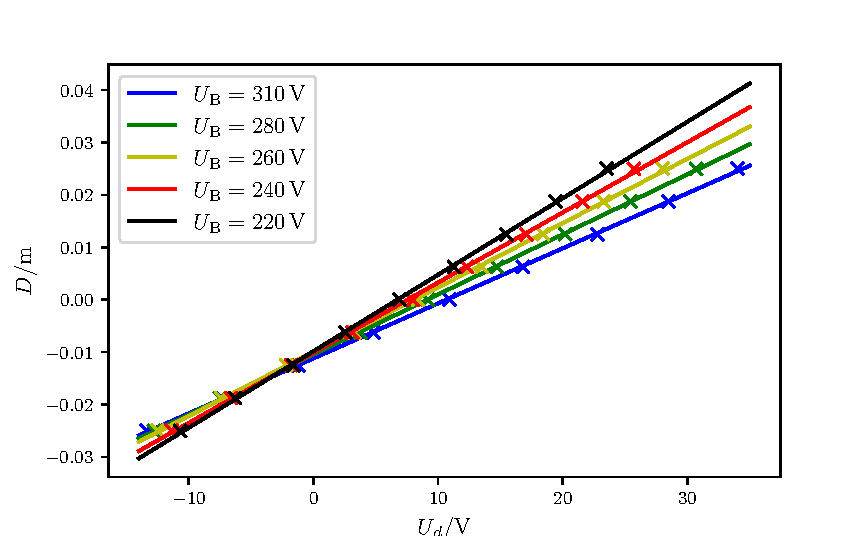
\includegraphics[width=\linewidth-70pt,height=\textheight-70pt,keepaspectratio]{content/images/GraphElek.pdf}
\caption{Das Verhältnis von Ablenkung $D$ zu Ablenkspannung $U_.d$ bei verschiedenen Beschleunigungsspannungen $U_.B$}\label{fig:Elek}
\end{figure}
\begin{figure}
\centering
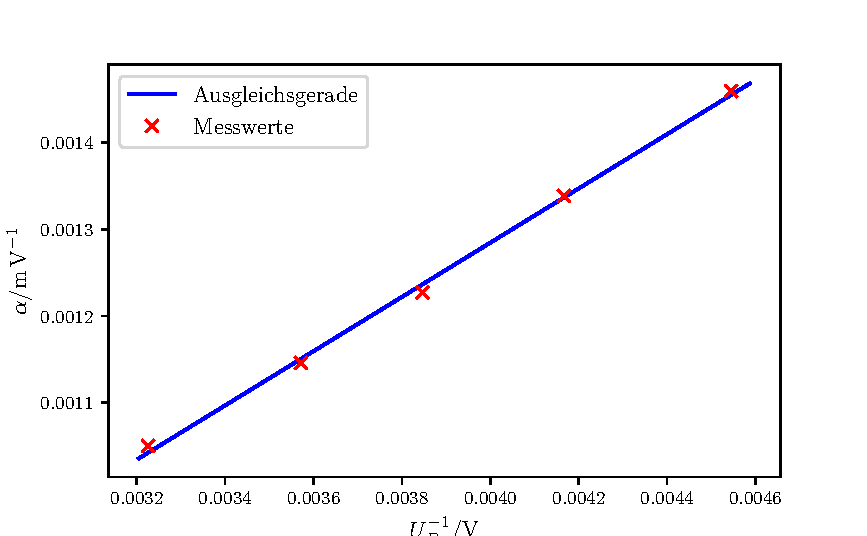
\includegraphics[width=\linewidth-70pt,height=\textheight-70pt,keepaspectratio]{content/images/GraphElek6.pdf}
\caption{Das Verhältnis der Empfindlichkeit $\alpha$ zu $\frac{1}{U_.B}$ bei verschiedenen Beschleunigungsspannungen $U_.B$}\label{fig:Elek2}
\end{figure}


\begin{table}
\centering
\caption{Messwerte der Sägezahnspannungen}
\label{tab:tabFreq}
	\sisetup{table-format=1.2}
	\begin{tabular}{S[table-format=1.1]S[table-format=2.2]S[table-format=2.2]}
		\toprule
		{$n$} & {$f_.{Säge}/\si{\hertz}$} & {$f_.{sin}/\si{\hertz}$} \\
		\midrule
		2.0 & 39.66 & 79.32 \\
		1.0 & 79.27 & 79.27 \\
		0.5 & 158.55 & 79.28 \\
		0.3 & 237.84 & 79.28 \\
		\bottomrule
	\end{tabular}

\label{tab:Freq}
\end{table}


\begin{table}
\centering
\caption{Messwerte der Ablenkungen bei verschiedenen Beschleunigungsspannungen $U_.B$}
\label{tab:tabMag}
	\sisetup{table-format=1.2}
	\begin{tabular}{S[table-format=2.2]S[table-format=1.2]S[table-format=1.2]S[table-format=2.2]S[table-format=1.2]S[table-format=2.2]}
		\toprule
		{$D/10^{-3}\si{\metre}$} & {$\frac{D}{D^2+L^2}/\si{\metre}$} & {$I_.{250}/\si{\ampere}$} & {$B_.{250}/10^{-5}\si{\tesla}$} & {$I_.{350}/\si{\ampere}$} & {$B_.{350}/10^{-5}\si{\tesla}$} \\
		\midrule
		6.25 & 0.20 & 0.30 & 1.91 & 0.41 & 2.61 \\
		12.50 & 0.41 & 0.63 & 4.02 & 0.83 & 5.29 \\
		18.75 & 0.61 & 0.95 & 6.06 & 1.20 & 7.65 \\
		25.00 & 0.80 & 1.30 & 8.29 & 1.60 & 10.20 \\
		31.25 & 0.99 & 1.60 & 10.20 & 2.00 & 12.75 \\
		37.50 & 1.17 & 1.95 & 12.44 & 2.40 & 15.31 \\
		43.75 & 1.34 & 2.35 & 14.99 & 2.85 & 18.17 \\
		50.00 & 1.51 & 2.70 & 17.22 & 3.20 & 20.41 \\
		\bottomrule
	\end{tabular}

\label{tab:Mag}
\end{table}